\setchaptergraphic{
    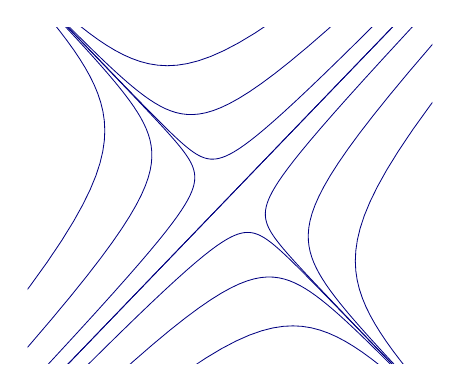
\begin{tikzpicture}[
        scale=0.75,
        declare function={f(\t) = 2*exp(-3*\t);
                          g(\t) = 4*exp(-3*\t);
                          s(\t) = 2*exp(\t);
                          d(\t) = -4*exp(\t);}
    ]
        \begin{axis}[
            ymin=-2,ymax=2,
            xmin=-1.25,xmax=1.25,
            hide axis,
        ]
        \foreach \h in {0.7,0.85,0.95,1.0}{
            \addplot[NavyBlue, domain=0:3, samples=60, variable=\t] plot ({\h*f(t)+(1.0-\h)*0.5*s(t)},{\h*g(t)+(1.0-\h)*0.5*d(t)});
            \addplot[NavyBlue, domain=0:3, samples=60, variable=\t] plot ({-\h*f(t)-(1.0-\h)*0.5*s(t)},{-\h*g(t)-(1.0-\h)*0.5*d(t)});
            \addplot[NavyBlue, domain=0:3, samples=60, variable=\t] plot ({-\h*f(t)+(1.0-\h)*0.5*s(t)},{-\h*g(t)+(1.0-\h)*0.5*d(t)});
            \addplot[NavyBlue, domain=0:3, samples=60, variable=\t] plot ({\h*f(t)-(1.0-\h)*0.5*s(t)},{\h*g(t)-(1.0-\h)*0.5*d(t)});
        }
        \end{axis}
    \end{tikzpicture}
}

\chapter{Ordinary Differential Equations}
\label{ch:diffeq}

\section{Classification}

\begin{defn}
    A \emph{differential equation} is an equation relating one or more independent variables, functions of those variables, and derivatives of those functions.
\end{defn}

\begin{exmp}\label{first-order-ode}
    \[\frac{\mathrm{d}x}{\mathrm{d}t} = x\]
\end{exmp}

\begin{defn}
    A \emph{solution} to a differential equation is an expression for the dependent functions of the differential equation in terms of the independent variables.
\end{defn}

Differential equations can be broadly classified into \emph{ordinary} and \emph{partial} differential equations.

\begin{defn}
    An \emph{ordinary} differential equation, or \emph{ODE} is a differential equation involving a single independent variable, and all derivatives are with respect to this variable.
\end{defn}

\begin{defn}
    A \emph{partial} differential equation, or \emph{PDE} is a differential equation involving functions of more than one independent variables, and derivatives may be with respect to any of those variables.
\end{defn}

\begin{defn}
    The \emph{general form} of an ODE is
    \[F(x, y, y', \ldots, y^{(n)}) = 0,\] that is some expression involving the independent variable $x$, the dependent variable $y$, and the derivatives of $y$.
\end{defn}

\begin{defn}
    The \emph{order} of a differential equation is the order of the highest derivative.
\end{defn}

\begin{exmp}
    \[\frac{\mathrm{d}^2\theta}{\mathrm{d}t^2} + \frac{g}{L}\sin\theta = 0\]
    This is a second order differential equation, while Example \ref{first-order-ode} is first order.
\end{exmp}

\begin{defn}
    A differential equation of a dependent variable $y$ and its derivatives is said to be \emph{linear} if it is an affine map with regard to $y$ and its derivatives.
\end{defn}

\begin{exmp}
    $\sin(x)y' + 2x^2y'' = x$ is linear.
\end{exmp}

\begin{exmp}
    $yy' + y'' = 0$ is non-linear.
\end{exmp}

\begin{defn}
    An \emph{autonomous} differential equation is one in which the independent variable does not explicitly appear. When the independent variable represents time in some way, these may also be called \emph{time-invariant}.
\end{defn}

\begin{exmp}
    $\frac{\mathrm{d}y}{\mathrm{d}x} = 5y - 20$ is an autonomous differential equation as the independent variable $x$ is not explicitly present.
\end{exmp}

\section{First order differential equations}

\begin{defn}
    The \emph{standard form} of a linear first order differential equation (with independent variable $t$ and dependent variable $y$) is \[\frac{\mathrm{d}y}{\mathrm{d}t} + p(t)y = g(t),\] for some arbitrary functions $p(t), g(t)$.
\end{defn}

Any linear first order autonomous ODE with independent variable $x$ and dependent variable $y$ can trivially be put into the form \[\frac{\mathrm{d}y}{\mathrm{d}x} = ay - b.\] This form can always be solved.

\begin{align*}
    \frac{\mathrm{d}y}{\mathrm{d}x} &= ay - b \\
    &= a(y - \frac{b}{a})
\end{align*}

Note that $\frac{\mathrm{d}}{\mathrm{d}x}{\left[y - \frac{b}{a}\right]} = \frac{\mathrm{d}}{\mathrm{d}x}y$. If $y \neq \frac{b}{a}$, we then have
\begin{align*}
    \frac{dy/dx}{y - b/a} = a,
\end{align*}
and so it follows that $\ln(y - \frac{b}{a}) = ax + C$ for some constant of integration $C$, so $\abs{y - \frac{b}{a}} = ke^{ax}$ for some $k$. If $y > \frac{b}{a}$, then $y = \frac{b}{a} + ke^{ax}$, and similarly if $y < \frac{b}{a}$, then $y = \frac{b}{a} + ke^{ax}$ for some $k$. In the case that $y = \frac{b}{a}$, it follows that $\frac{\mathrm{d}y}{\mathrm{d}x} = 0$, so $y = \frac{b}{a} + ke^{ax}$ where $k = 0$.

Therefore, $y = \frac{b}{a} + ke^{ax}$ is a solution to any linear first order autonomous differential equation.

\subsection{Linear equations}

Linear first order ODEs which are not autonomous can sometimes be solved through the use of an \emph{integrating factor}. We can write a linear first order ODE as \[y' + p(t)y = g(t),\] where $p(t), g(t)$ are arbitrary functions. Our goal here is to find a function $\mu(t)$, called the \emph{integrating factor}, such that
\[\frac{\mathrm{d}}{\mathrm{d}t}\mu(t)y = \mu(t)y' + p(t)\mu(t)y.\] That is, we want $\mu'(t) = p(t)\mu(t)$. Once such $\mu(t)$ is found, since \[\mu(t)y' + \mu(t)p(t)y = \mu(t)g(t),\] we clearly have \[\frac{\mathrm{d}}{\mathrm{d}t}\mu(t)y = \mu(t)g(t).\] It follows that \[y = \frac{1}{\mu(t)}\int_{t_0}^t \mu(s)g(s)ds + C\] for some constants $t_0$ and $C$.

We of course need to also be able to find such a $\mu(t)$. Note that since $\mu'(t) = p(t)\mu(t)$ we have \[\frac{\mu'(t)}{\mu(t)} = p(t).\] Since $\frac{\mathrm{d}}{\mathrm{d}t}\ln(\mu(t)) = \frac{\mu'(t)}{\mu(t)}$, it follows that $\ln(\mu(t)) = \int p(t)$. Therefore, $\mu(t) = e^{\int p(t)dt}$.

\begin{exmp}
    Using an integrating factor to solve $ty' + 2y = 4t^2$ with the initial condition $y(1) = 2$.

    First, we need the differential equation in the standard form $y' + p(t)y = g(t)$. Doing this, we obtain $y' + \frac{2}{t}y = 4t$, provided that $t \neq 0$. Then we have $\ln(\mu(t)) = \int \frac{2}{t}dt = 2\ln(t) = \ln(t^2)$, so $\mu(t) = t^2$. We know have $\frac{\mathrm{d}}{\mathrm{d}t}\mu(t)y = 4t^3$, which we may integrate to obtain $t^2y = t^4 + c$, and so $y = t^2 + \frac{c}{t^2}$. Applying the initial condition $y(1) = 2$, we have $2 = 1 + c$, so $c = 1$ and our final particular solution is \[y = t^2 + \frac{1}{t^2}, t > 0.\]
\end{exmp}

\subsection{Separable equations}

A separable first order differential equation is of the form
\[\frac{\mathrm{d}y}{\mathrm{d}t} = g(t)h(y),\] so that we may ``separate'' the independent and dependent variables to obtain
\[\frac{1}{h(y)}\frac{\mathrm{d}y}{\mathrm{d}t} = g(t).\] This can be often be integrated, with the particularly nice property that due to the chain rule, we can simply integrate the LHS with respect to $y$.
\[\int \frac{1}{h(y)}dy = \int g(t)dt.\] These integrals may or may not be computable, and even if they are the resulting equation may not be solvable for $y$. However, it can sometimes be done and is a simple and straightforward technique.

\subsection{Autonomous equations}

In general, any first order autonomous ODE is of the form $\frac{dy}{dt} = f(y)$. Note that this form is always separable.

\begin{rmk}
    Note that the slope field of every autonomous ODE has the same slope for any given value of $y$, regardless of $t$.
\end{rmk}

\begin{defn}
    Let $y' = f(y)$ be a first order autonomous ODE, and consider the set
    \[\left\{y \in \R \compbar f(y) = 0 \right\}.\]
    This is the \emph{critical point} set of the ODE.
\end{defn}

\begin{defn}
    Let $y' = f(y)$ be a first order autonomous ODE. For any $y_{\star}$ in the critical point set, $y(t) = y_{\star}$ is an \emph{equilibrium solution} to the ODE.
\end{defn}

\begin{exmp}
    Let $y' = y(1-y)$. The polynomial $y(1-y)$ is zero when $y = 0$ or $y = 1$, so $y(t) = 0$ and $y(t) = 1$ are equilibrium solutions.
\end{exmp}

\begin{rmk}
    In between equilibria, the sign of $y'$ does not change.
\end{rmk}

\begin{rmk}
    Given a first order autonomous ODE $y' = f(y)$, since the sign of $y'$ goes not change between critical points, we can use the sign of $y''$(which is also $f'(y)$) to learn more about the behavior of solutions around critical points.
\end{rmk}

\begin{defn}
    Let $y' = f(y)$ be a first order autonomous ODE. If $f(y) > 0$ at a critical point $y_{\star}$, then when $y > y_{\star}$ the solution increases and when $y < y_{\star}$ the solution decreases. That is, solutions near the equilibrium of the critical point diverge from it, so we call these \emph{unstable} equilibria. Similarly, if $f'(y_{\star}) < 0$ then nearby solutions converge towards $y_{\star}$, and so we call it a \emph{stable} equilibrium.
\end{defn}

\begin{rmk}
    Stable equilibria are also called \emph{sinks}, while unstable equilibria may be called \emph{sources}.
\end{rmk}

\begin{exmp}
    Let $y' = (1-y)^2(y-4)$, and so $y'' = -2(1-y)(y-4) + (1-y)^2$. Since both $y'$ and $y''$ are continuous on $\R$, by Theorem \ref{general-first-order-existence} we know that a unique solution must exist for any given initial value. It follows that no solution curves cross each other anywhere.

    Furthermore, we can see that the critical points are $1$ and $4$, and since $y''(4) = 9$ and $y''(1) = 0$ it follows that $4$ is an unstable equilibrium. We know that $1$ is an equilibrium as well, and that $y''' < 0$, so $1$ is semi-stable --- solutions converge to it from above, and diverge from it below.
\end{exmp}

\subsection{Existence and uniqueness of solutions}

\begin{thm}\label{linear-first-order-existence}
    Let $I = (\alpha, \beta)$ be an open interval containing $t = t_0$, and let $p, g$ be functions that are continuous on $I$. There exists a unique function $y(t)$ that satisfies both the differential equation
    \[\frac{dy}{dt} + p(t)y = g(t)\] and the initial condition $y(t_0) = y_0$ for some $y_0$.
\end{thm}

\begin{proof}
    Since the differential equation is linear, it can be solved using an integrating factor, and the initial condition uniquely determines the constant of integration.
\end{proof}

\begin{thm}\label{general-first-order-existence}
    Let the functions $f$ and $\frac{\partial{f}}{\partial{y}}$ be continuous in some rectangular region $\alpha < t < \beta, \gamma < y < \delta$ containing a point $(t_0, y_0)$. Then, for some interval $(t_0 - h, t_0 + h)$ within $(\alpha, \beta)$, there exists a unique function $y(t)$ that satisfies both the differential equation
    \[\frac{dy}{dt} = f(t, y)\] and the initial condition $y(t_0) = y_0$.
\end{thm}

\begin{cor}
    The continuity of $f$ alone is sufficient for the existence of solutions, but not their uniqueness.
\end{cor}

\begin{rmk}
    Note that Theorem \ref{general-first-order-existence} ensures two solutions cannot intersect each other, since the differential equation with initial condition corresponding to the intersection would be satisfied by both solutions.
\end{rmk}

\begin{exmp}
    Consider $\dot{z} = z(1-z)$. Since $z(1-z)$ is a polynomial, it is continuous for all $z$, and so is $\frac{d}{dz}z(1-z)$. By Theorem \ref{general-first-order-existence}, it therefore has a unique solution for any given initial value.
\end{exmp}

\begin{exmp}
    Consider $y(t) = y^{2/3}$. Since $y^{2/3}$ is continuous for all $y$, the \emph{existence} of a solution is guaranteed for all initial values by Theorem $\ref{general-first-order-existence}$. However, since $\frac{d}{dy}y^{2/3} = \frac{2}{3}y^{-1/3}$ is discontinuous at $y = 0$, the \emph{uniqueness} of the solution is only guaranteed for initial values $y \neq 0$.
\end{exmp}

\begin{exmp}
    Consider $\dot{x} = \sqrt{x}$. Since $\sqrt{x}$ is only continuous for $x > 0$, given the initial condition $x(0) = x_0$, neither the existence nor uniqueness of a solution is not guaranteed.
\end{exmp}

\subsection{Exact equations}

\begin{defn}
    A first order ODE of the form $M(x, y) + N(x, y)y' = 0$ (where $y$ is a function of $x$) is \emph{exact} if there exists some function $\psi(x, y)$ such that $\frac{d\psi}{dx} = M(x, y) + N(x, y)y'$.
\end{defn}

\begin{exmp}
    $2x + y^2 + 2xyy' = 0$ is an exact first order ODE, since $\psi(x, y) = x^2 + xy^2$ gives $\frac{d\psi}{dx} = 2x + y^2 + 2xyy' = 0$. It follows that $\psi(x, y) = \int{0}dx$, and so $x^2 + xy^2 = c$ for some constant $c$ is a solution.
\end{exmp}

\begin{thm}
    Let functions $M, N, M_y, N_x$ be continuous on a simply connected region in the $xy$ plane. Then $M(x, y) + N(x, y)y' = 0$ is an exact differential equation if and only if $M_x(x, y) = N_y(x, y)$ for all points on the region.
\end{thm}

\begin{proof}\proofbreak
    ($\implies$) If it is an exact differential equation, then by definition there exists some $\psi(x, y)$ such that $\psi_x(x, y) = M(x, y)$ and $\psi_y(x, y) = N(x, y)$. Therefore, $\psi_{xy}(x, y) = M_y(x, y)$ and $\psi_{yx} = N_x(x, y)$. Since $M_y, N_x$ are continuous are some region, $\psi$ is $C^2$ are that region, and so $\psi_{xy} = \psi_{yx}$, implying $M_y = N_x$.

    ($\impliedby$) Since $M$ is continuous on the region, we can integrate to obtain $\varPhi(x, y) = Q(x, y) + h(y)$, where $\frac{d}{dx}Q = M$ and $h(y)$ is an arbitrary function. We need $\frac{d}{dx}\varPhi(x, y) = M(x, y) + N(x, y)y'$, so we need to be able to choose $h(y)$ such that $\frac{d}{dy}\varPhi = N(x,y)$. We therefore have $\frac{d}{dy}\varPhi = \frac{d}{dy}Q + h'(y) = N(y)$, and so $h'(y) = N(y) - \frac{d}{dy}Q$. This equation is integrable (giving a solution for $h(y)$) when $N(x,y) - \frac{d}{dy}Q(x,y)$ is solely a function of $y$. Since $\frac{d}{dx}\left(N(x,y) - \frac{d}{dy}Q(x,y)\right) = N_x - M_y = 0$, it is not a function of $x$, and so there is function $\varPhi(x,y)$ such that $\frac{d}{dy}\varPhi = N(x,y)$ and $\frac{d}{dx}\varPhi = M(x,y)$.
\end{proof}

\begin{exmp}
    Consider the first order differential equation \[\left(3x^2 - 2xy + 2\right) + \left(6y^2 - x^2 + 3\right)y' = 0.\] Since $\frac{d}{dy}\left(3x^2 - 2xy + 2\right) = -2x$ and $\frac{d}{dx}\left(6y^2 - x^2 + 3\right) = -2x$, this is an exact differential equation.
    \[\int \left(3x^2 - 2xy + 2\right)dx = x^3 - x^2y + 2x + h(y).\] Since $\frac{d}{dy}\left(x^3 - x^2y + 2x\right) = -x^2$, we then want $h'(y) = \left(6y^2 - x^2 + 3\right) - (-x^2) = 6y^2 + 3$. Then, $h(y) = \int h'(y)dy = 2y^3 + 3y$, and so the general solution is \[\psi(x, y) = x^3 - x^2y + 2x + 2y^3 + 3y = c.\]
\end{exmp}

\begin{rmk}
    Some non-exact first order differential equations can be made exact by way of an integrating factor.
\end{rmk}

\begin{exmp}
    Consider the differential equation $1 + \left(\frac{x}{y}- \sin(y)\right)y' = 0$. This is clearly not exact, but multiplying the equation by the integrating factor $y$ results in $y + \left(x - y\sin(y)\right)y' = 0$, which is exact and can be solved.
\end{exmp}

\begin{prop}
    All separable first order differential equations are exact.
\end{prop}

\begin{proof}
    Let $y' = g(y)h(x)$ be a separable equation. Then $-h(x) + \frac{1}{g(y)}y' = 0$. Since $\frac{\partial}{\partial y}\left(-h(x)\right) = 0 = \frac{\partial}{\partial}\frac{1}{g(y)}$, this is an exact differential equation.
\end{proof}

\section{Linear second order equations}

\subsection{Homogeneous equations with constant coefficients}

Let $ay'' + by' + cy = 0$ be a homogeneous second order differential equation, where $a, b, c$ are constants. Notice that if $y = e^{rt}$ for some $r$, then $a'' + by' + cy = ar^2e^{rt} + bre^{rt} + ce^{rt} = (ar^2 + br + c)e^{rt} = 0$. Since $e^{rt} \neq 0$, it follows that $ar^2 + br + c = 0$, and so $y = e^{rt}$ is a solution when $r$ is a root of $ar^2 + br + c = 0$. Furthermore, notice that any linear combination of solutions is also a solution, since the differential equation is homogeneous.

\begin{defn}
    For a differential equation of the form $ay'' + by' + cy = 0$, the equation $ar^2 + br + c = 0$ is called the \emph{characteristic equation}.
\end{defn}

\begin{exmp}
    Consider the constant coefficient homogeneous differential equation $2y'' + 8y' - 10y = 10$. We know that $y = e^{rt}$ is a solution when $r$ is a root of $2r^2 + 8r - 10$, and since $2r^2 + 8r - 10 = (2r-2)(r+5)$, this gives us $r = 1, -5$. The general solution is then $y(t) = c_1e^t + c_2e^{-5t}$ for some constants $c_1, c_2 \in \R$.

    Given two initial conditions, we can solve for $c_1$ and $c_2$. For example, if $y(0) = 2$ and $y'(0) = -4$, we have $2 = c_1 + c_2$ and $-4 = c_1 - 5c_2$. This system can be solved, yielding $6 = 6c_2$, so $c_2 = 1$ and so $c_1 = 1$ as well.
\end{exmp}

\begin{defn}
    For functions $p(t), q(t)$, define the operator $L$ as
    \[L[\phi] = \frac{d^2}{dt^2}\phi + p(t)\frac{d}{dt}\phi + q(t)\phi.\]
\end{defn}

\begin{thm}\label{linear-second-order-existence}Existence and Uniqueness\proofbreak
    Consider the initial value problem $L[y] = g(t)$, with $y(t_0) = y_0$ and $y'(t_0) = y_0'$. If $p(t)$, $q(t)$, and $g(t)$ are continuous on an open interval $I$ where $t_0 \in I$, then there is exactly one solution to this problem, and it is defined for all of $I$.
\end{thm}

\begin{exmp}
    Consider $L[y] = 0$, $y(t_0) = 0$, and $y'(t_0) = 0$, where $p(t), q(t)$ are continuous on an open interval containing $t_0$. Then since $\phi(t) = 0$ is a solution, by Theorem \ref{linear-second-order-existence} this is the only solution.
\end{exmp}

\begin{thm}\label{linear-superposition}Superposition\proofbreak
    For $L[y] = 0$, let $y_1, y_2$ be solutions. Then $c_1y_1 + c_2y_2$ are solutions for any $c_1, c_2 \in \R$.
\end{thm}

\begin{proof}
    Let $\phi = c_1y_1 + c_2y_2$, then $\phi' = c_1y_1' + c_2y_2'$ and $\phi'' = c_1y_1'' + c_2y_2''$. Therefore,
    \begin{align*}
        L[\phi] &= \phi'' + p(t)\phi' + q(t)\phi \\
        &= (c_1y_1'' + c_2y_2'') + p(t)(c_1y_1' + c_2y_2') + q(t)(c_1y_1 + c_2y_2) \\
        &= c_1(y_1'' + p(t)y_1' + q(t)y_1) + c_2(y_2'' + p(t)y_2' + q(t)y_2) \\
        &= c_1L[y_1] + c_2L[y_2].
    \end{align*}
    Since $y_1, y_2$ are solutions to $L[y] = 0$, we then know that $L[\phi] = c_1(0) + c_2(0) = 0$, and so it is also a solution.
\end{proof}

\begin{defn}
    For functions $y_1, y_2$, the \emph{Wronskian determinant} is the determinant of the coefficient matrix of the system of equations
    \begin{align*}
        c_1y_1(t_0) + c_2y_2(t_0) = y_0, \\
        c_1y_1'(t_0) + c_2y_2'(t_0) = y_0',
    \end{align*}
    and is given by
    \[W = y_1y_2' - y_1'y_2\] at $t_0$.
\end{defn}

\begin{thm}\label{linear-initial-conditions-existence}
    For $L[y] = 0$, let $y_1, y_2$ be solutions. Given the initial conditions $y(t_0) = y_0$ and $y'(t_0) = y_0'$, there exists $c_1, c_2$ such that $y = c_1y_1 + c_2y_2$ is a solution satisfying the initial conditions if and only if the Wronskian $W = y_1y_2' - y_1'y_2$ is non-zero at $t_0$.
\end{thm}

\begin{thm}\label{linear-second-order-solution-family}
    For $L[y] = 0$, let $y_1, y_2$ be solutions. The family of solutions described by $y = c_1y_1 + c_2y_2$ includes every possible solution to $L[y] = 0$ if and only if there exists $t_0$ such that the Wronskian is non-zero at $t_0$.
\end{thm}

\begin{proof}
    Let $t_0$ be such that the Wronskian is non-zero at $t_0$, and let $\phi$ be any solution to $L[y] = 0$. Let $y_0 = \phi(t_0)$ and $y_0' = \phi'(t_0)$. Then by Theorem \ref{linear-initial-conditions-existence}, there exists some $c_1, c_2$ such that $c_1y_1 + c_2y_2$ is a solution to $L[y] = 0$ satisfying $y(t_0) = y_0$ and $y'(t_0) = y_0'$. Then by Theorem \ref{linear-second-order-existence}, this is the only such solution, and so it must be that $\phi = c_1y_1 + c_2y_2$.

    Now consider the case where no such $t_0$ exists. Then by Theorem \ref{linear-initial-conditions-existence} there exist initial conditions such that no linear combination of $y_1, y_2$ satisfy them. However, by Theorem \ref{linear-second-order-existence} there is a unique solution satisfying these conditions, and so that solution cannot be in the family $c_1y_1 + c_2y_2$.
\end{proof}

\begin{prop}
    Let $y_1 = e^{r_1t}, y_2 = e^{r_2t}$ be solutions to $L[y] = 0$. Then $c_1y_1 + c_2y_2$ describe all possible solutions if and only if $r_1 \neq r_2$.
\end{prop}

\begin{proof}
    The Wronskian is given by $y_1y_2' - y_1'y_2 = r_2e^{r_1t}e^{r_2t} = r_1e^{r_1t}e^{r_2t}$, so the Wronskian is non-zero precisely when $r_1 \neq r_2$. Then by Theorem \ref{linear-second-order-solution-family}, $c_1y_1 + c_2y_2$ describe all possible solutions if and only if $r_1 \neq r_2$.
\end{proof}

\begin{thm}\label{family-basis-exists}
    Consider $L[y] = 0$ where $p(t), q(t)$ are continuous on some open interval $I$. Fix some $p_0 \in I$. Let $y_1$ be the unique solution that satisfies $y(t_0) = 1$ and $y'(t_0) = 0$, and let $y_2$ be the unique solution which satisfies $y(t_0) = 0$ and $y'(t_0) = 1$. Then linear combinations of $y_1$ and $y_2$ describe all possible solutions to $L[y]$.
\end{thm}

\begin{proof}
    Note that $y_1, y_2$ are guaranteed to exist and be unique on $I$ by Theorem \ref{linear-second-order-existence}. At $t_0$, the Wronskian is given by $W = y_1(t_0)y_2'(t_0) - y_1'(t_1)y_2(t_0) = 1(1) - 0(0) = 1$. Since $W \neq 0$, by Theorem \ref{linear-second-order-solution-family} linear combinations of $y_1, y_2$ describe all possible solutions.
\end{proof}

\begin{thm}\label{abels-thm}Abel's Theorem\proofbreak
    Let $y_1, y_2$ be solutions to $L[y] = 0$, where $p(t, q(t))$ are continuous on some open interval $I$. Then the Wronskian is given by \[W(t) = c\exp\left(-\int p(t)dt\right)\] for some constant $c$.
\end{thm}

\begin{proof}
    We know that
    \begin{align*}
        y_1'' + p(t)y_1' + q(t)y_1 &= 0, \\
        y_2'' + p(t)y_2' + q(t)y_2 &= 0.
    \end{align*}
    Multiplying these equations by $y_2$ and $y_1$ respectively and then subtracting, we obtain
    \[(y_1''y_2 - y_1y_2'') + p(t)(y_1'y_2 - y_1y_2') + q(t)(y_1y_2 - y_1y_2).\] Note that the Wronskian is $W = y_1'y_2 - y_1y_2'$, and that
    \[W' = y_1''y_2 + y_1'y_2' - y_1'y_2' - y_1y_2'' = y_1''y_2 - y_1y_2''.\]
    Therefore, we have $W' + p(t)W = 0$. This is a first order linear differential equation, which we can solve with the integrating factor $\exp\left(\int p(t)dt\right)$, giving us $W(t) = c\exp\left(-\int p(t)dt\right)$ for some constant $c$.
\end{proof}

\begin{cor}\label{wronskian-always-zero}
    The Wronskian is either always zero or always non-zero.
\end{cor}

\begin{proof}
    Since $\exp\left(-\int p(t)dt\right) \neq 0$, we know that the Wronskian is only zero if $c = 0$, in which case it is always zero.
\end{proof}

\subsection{Complex roots of the characteristic equation}

\begin{thm}\label{complex-solution-decomposition}
    Consider $L[y] = 0$. If $y(t) = u(t) + iv(t)$ is a complex-valued solution, then $u(t)$ and $v(t)$ are also solutions.
\end{thm}

\begin{proof}
    Since $y(t)$ is a solution, we know that
    \begin{align*}
        0 = L[y] &= (u''(t) + iv''(t)) + p(t)(u'(t) + iv'(t)) + q(t)(u(t) + iv(t)) \\
        &= (u''(t) + p(t)u'(t) + q(t)u(t)) + i(v''(t) + p(t)v'(t) + q(t)v(t)) \\
        &= L[u] + iL[v].
    \end{align*}
    It follows that $L[u] = 0 = L[v]$.
\end{proof}

\begin{exmp}
    Consider $y'' + y' + \frac{37}{4}y = 0$, with the initial conditions $y(0) = 2$ and $y'(0) = 8$.

    The roots of the characteristic equation are \[r = \frac{-1 \pm \sqrt[]{1 - 37}}{2} = -\frac{1}{2} \pm 3i.\] Since $e^{rt}$ is a solution, we know that $\exp\left(-\frac{1}{2}t + 3it\right)$ is a solution. By Euler's formula, \[\exp\left(-\frac{1}{2}t + 3it\right) = e^{-t/2}e^{3it} = e^{-t/2}\cos(3t) + ie^{-t/2}\sin(3t).\] Then by Theorem \ref{complex-solution-decomposition}, $u(t) = e^{-t/2}\cos(3t)$ and $v(t) = e^{-t/2}\sin(3t)$ are real-valued solutions. The Wronskian of these solutions is $W(u, v) = 3e^{-t}$, which is non-zero so by Theorem \ref{linear-second-order-solution-family} linear combinations are $u$ and $v$ describe all possible (even complex-valued) solutions.

    For the specific initial conditions $y(0) = 2$ and $y'(0) = 8$, we find $c_1e^{0}\cos(0) + c_2e^{0}\sin(0) = 2$ implies $c_1 = 2$, and $c_1(-\frac{1}{2}e^{0}\cos(0) - 3e^{0}\sin(0)) + c_2(-\frac{1}{2}e^{0}\sin(0) + 3e^{0}\cos(0))$, so $-1 + 3c_2 = 8$, and so $c_2 = 3$. Therefore, our solution is \[y = 2e^{-t/2}\cos(3t) + 3e^{-t/2}\sin(3t).\]
\end{exmp}

\begin{prop}
    Let $ay'' + by' + cy = 0$ be a differential equation whose characteristic equation has complex roots $r_1, r_2$. If we decompose $r_1$ (or $r_2$) into $\lambda + i\mu$, then linear combinations of $e^{\lambda}\cos(\mu{t})$ and $e^{\lambda}\sin(\mu{t})$ describe all possible solutions.
\end{prop}

\begin{proof}
    Since $e^{r_1t}$ is a solution, by Theorem \ref{complex-solution-decomposition} we know that $e^{\lambda}\cos(\mu{t})$ and $e^{\lambda}\sin(\mu{t})$ are also solutions. The Wronskian is
    \[W = e^{2\lambda}\mu.\] Since $\lambda \in \R$, we know that $e^{2\lambda} < 0$, and since $r_1 \notin \R$, we know that $\mu \neq 0$. Therefore, $W \neq 0$. By Theorem \ref{linear-second-order-solution-family}, linear combinations of $e^{\lambda}\cos(\mu{t})$ and $e^{\lambda}\sin(\mu{t})$ describe all positions solutions.
\end{proof}

\subsection{Repeated roots of the characteristic equation}

Given the differential equation $ay'' + by' + cy = 0$, when $b^2 - 4ac = 0$ the characteristic equation has a repeated root $r$, giving the solution $e^{rt}$. To describe all possible solutions we need two distinct solutions whose Wronskian is non-zero.

For any solution $y_1 = e^{rt}$ and arbitrary constant $c$, we know that $ce^{rt}$ is also a solution. To find a second solution, we can try generalizing this to $\phi(t) = v(t)e^{rt}$ and attempt to find a function $v(t)$ such that $\phi(t)$ is a solution. We can see that $\phi' = v'(t)e^{rt} + rv(t)e^{rt}$ and $\phi'' = v''(t)e^{rt} + 2rv'(t)e^{rt} + r^2v(t)e^{rt}$. Note that $r = -\frac{b}{2a}$, so
\begin{align*}
    \phi &= e^{rt}v(t) \\
    \phi' &= e^{rt}(v'(t) - \frac{b}{2a}v(t)) \\
    \phi'' &= e^{rt}(v''(t) - \frac{b}{a}v'(t) + \frac{b^2}{4a^2}v(t)).
\end{align*}
For $\phi$ to be a solution, it must satisfy $a\phi'' + b\phi' + c\phi = 0$. Since $e^{rt}$ is a common factor to each term and is non-zero, we can divide it out and rearrange to obtain
\[av''(t) - bv'(t) + \frac{b^2}{4a}v(t) + bv'(t) - \frac{b^2}{2a}v(t) + cv(t) = 0,\] and so $av''(t) - \left(\frac{b^2}{4a} - c\right)v(t) = 0$. Note that since $b^2 - 4ac = 0$, we have $\frac{b^2}{4a} - c = 0$. Therefore, $av''(t) = 0$, and so $v''(t) = 0$. It follows that $v(t) = c_1t + c_2$ for some constants $c_1, c_2$. Therefore, $y = c_1te^{rt} + c_2e^{rt}$ is a solution for any $c_1, c_2$.

\begin{thm}\label{linear-second-order-repeated-roots}
    Let $ay'' + by' + cy = 0$ be a differential equation whose characteristic equation has a repeated root $r$. Then linear combinations of $e^{rt}$ and $te^{rt}$ describe all possible solutions.
\end{thm}

\begin{proof}
    The Wronskian is \[W = e^{rt}(e^{rt} + te^{rt}) - te^{rt}(e^{rt}) = e^{2rt},\] which is non-zero since $r \in \R$. Therefore, by Theorem \ref{linear-second-order-solution-family} linear combinations of $e^{rt}$ and $te^{rt}$ describe all possible solutions.
\end{proof}

\begin{rmk}
    The method used to find the second solution in the same of the repeated root can be used to find a second solution from another solution for a linear second order differential equation.
\end{rmk}

\begin{prop}\label{reduction-of-order}
    Given a solution $y_1(t)$ to $y''(t) + p(t)y' + q(t)y = 0$, another solution $y_2(t)$ of the form $v(t)y_1(t)$ must satisfy the \emph{first-order linear} differential equation
    \[y_1v'' + \left(2y_1' + p(t)y_1\right)v' = 0.\]
\end{prop}

\begin{proof}
    \begin{align*}
        y_2' &= v'y_1 + vy_1' \\
        y_2'' &= v''y_1 + 2v'y_1' + vy_2''.
    \end{align*}
    Substituting $y_2(t)$ into the differential equation we then obtain
    \begin{align*}
        0 &= y_2'' + p(t)y_2' + q(t)y_2 \\
        &= \left(v''y_1 + 2v'y_1' + vy_1''\right) + p(t)\left(v'y_1 + vy_1'\right) + q(t)vy_1 \\
        &= y_1v'' + \left(2y_1' + p(t)y_1\right)v' + \left(y_1'' + p(t)y_1' + q(t)y_1\right)v.
    \end{align*}
    Since $y_1$ is a solution, $y_1'' + p(t)y_1' + q(t)y_1 = 0$ so this reduces to
    \begin{align*}
        y_1v'' + \left(2y_1' + p(t)y_1\right)v' = 0.
    \end{align*}
\end{proof}

\begin{prop}
    Let solutions $y_1(t)$ and $y_2(t) = v(t)y_1(t)$ as in Proposition \ref{reduction-of-order}, then $y_1(t)$ and $y_2(t)$ are linearly independent whenever $v'$ is non-zero.
\end{prop}

\begin{exmp}
    Let $2t^2y'' + 3ty' - y = 0$, where $t > 0$ and $y(t) = t^{-1}$ is a known solution. Then we try $\phi(t) = v(t)y(t)$ for some $v(t)$, and so $\phi'(t) = v(t)y'(t) + v'(t)y(t) = v'(t)t^{-1} - v(t)t^{-2}$. Similarly, $\phi''(t) = v'(t)y'(t) + v(t)y''(t) + v''(t)y(t) + v'(t)y'(t)$, so we have
    \begin{align*}
        \phi &= t^{-1}v(t) \\
        \phi' &= v'(t)t^{-1} - v(t)t^{-2} \\
        \phi'' &= -v'(t)t^{-2} + 2v(t)t^{-3} + v''(t)t^{-1} - v'(t)t^{-2}.
    \end{align*}
    From the differential equation, we then have
    \begin{align*}
        0 &= 2t^2\phi'' + 3t\phi' - \phi \\
        &= -2v'(t) + 4t^{-1}v(t) + 2tv''(t) - 2v'(t) + 3v'(t) - 3t^{-1}v(t) - t^{-1}v(t) \\
        &= 2tv''(t)-v'(t) = 0.
    \end{align*}
    Note that this is equivalent to the first order linear differential equation of $v'(t)$, so $\mu(t) = \exp\left(-\frac{1}{2}\ln(t)\right) = t^{-1/2}$, and so $v'(t) = c_1\sqrt{t}$. Therefore,
    \[v(t) = c_1\int t^{1/2}dt = \frac{2}{3}c_1t^{3/2} + c_2.\] Finally, we obtain
    \[\phi(t) = v(t)t^{-1} = \frac{2}{3}c_1t^{1/2} + c_2t^{-1}.\] Since we already had $y(t) = t^{-1}$, our solutions become $y_1(t) = t^{-1}, y_2(t) = t^{1/2}$.

    Since the Wronskian is
    \[W = \frac{1}{2}t^{-3/2} + t^{-3/2} = \frac{3}{2}t^{-3/2},\] and we know $t > 0$, the Wronskian is non-zero and so these solutions are linearly independent.
\end{exmp}

\subsection{Nonhomogeneous equations}

\begin{defn}
    For a linear nonhomogeneous differential equation
    \[L[y] = y'' + p(t)y' + q(t)y = g(t),\] then the equation
    \[L[y] = y'' + p(t)y' + q(t)y = 0\] is called the \emph{corresponding homogeneous equation}.
\end{defn}

\begin{thm}\label{linear-nonhomogeneous-sum}
    If $Y_1(t)$ and $Y_2(t)$ are solutions to
    \begin{align*}
        ay'' + by' + cy &= g_1(t), \\
        ay'' + by' + cy &= g_2(t)
    \end{align*} respectively, then $c_1Y_1(t) + c_1Y_2(t)$ is a solution to
    \[ay'' + by' + cy = c_1g_1(t) + c_2g_2(t).\]
\end{thm}

\begin{proof}
    Let $Y(t) = c_1Y_1(t) + c_2Y_2(t)$. Then
    \begin{align*}
        aY'' + bY' + cY &= a(c_1Y_1'' + c_1Y_2'') + b(c_1Y_1' + c_1Y_2') + c(c_1Y_1 + c_1Y_2) \\
        &= c_1\left(aY_1'' + bY_1' + cY_1\right) + c_2\left(aY_2'' + bY_2' + cY_2\right) \\
        &= c_1g_1(t) + c_2g_2(t).
    \end{align*}
\end{proof}

\begin{cor}\label{linear-second-order-nonhomogeneous-difference}
    If $Y_1(t), Y_2(t)$ are solutions to a nonhomogeneous equation, and $y_1(t), y_2(t)$ are linearly independent solutions to the corresponding homogeneous equation, then for some $c_1, c_2$
    \[Y_1(t) - Y_2(t) = c_1y_1(t) + c_2y_2(t).\]
\end{cor}

\begin{proof}
    By Theorem \ref{linear-nonhomogeneous-sum}, $Y_1(t) - Y_2(t)$ is a solution to $L[y] = g_1(t) - g_2(t) = 0$. By Theorem \ref{linear-second-order-solution-family}, all such solutions are equal to $c_1y_1(t) + c_2y_2(t)$ for some $c_1, c_2$.
\end{proof}

\begin{thm}\label{linear-second-order-general-solution}
    If $y_1(t), y_2(t)$ satisfy $L[y] = 0$ and are linearly independent, and $Y(t)$ is a solution to $L[y] = g(t)$, then $y = c_1y_1(t) = c_2y_2(t) + Y(t)$ is a general solution to $L[y] = g(t)$.
\end{thm}

\begin{proof}
    Let $Y'(t)$ be any solution to $L[y] = g(t)$. Then by Corollary \ref{linear-second-order-nonhomogeneous-difference}, $Y'(t) - Y(t) = c_1y_1(t) + c_2y_2(t)$ for some $c_1, c_2$, and so $Y'(t) = c_1y_1(t) + c_2y_2(t) + Y(t)$.
\end{proof}

\begin{rmk}
    As a consequence of Theorem \ref{linear-second-order-general-solution}, to solve a linear second order nonhomogeneous differential equation, we need to first solve the corresponding homogeneous equation, and also find one particular solution to the nonhomogeneous equation.
\end{rmk}

\begin{defn}
    The \emph{method of undetermined coefficients} is one strategy to find a particular solution to a nonhomogeneous differential equation. By guessing that $Y(t)$ takes a similar form to the nonhomogeneous term, but with undetermined variable coefficients, it is sometimes possible to determine possible values for those coefficients.
\end{defn}

\begin{exmp}
    To find a particular solution to $y'' - 3y' - 4y = 2\sin(t)$, we might initially guess $Y(t) = A\sin(t)$ for some $A$. Then $Y' = A\cos(t)$ and $Y'' = -A\sin(t)$, and so we have $-A\sin(t) - 3A\cos(t) - 4A\sin(t) = 2\sin(t)$, and so $(2 + 5A)\sin(t) + 3A\cos(t) = 0$. At $t = 0$ this implies $3A = 0$ and at $t = \frac{\pi}{2}$ this implies $2 + 5A = 0$, but there is no such $A$, so our guess was wrong.

    Noting that that our result contained both sine and cosine, we instead now guess that $Y = A\sin(t) + B\cos(t)$, and so $-A\sin(t) - B\cos(t) - 3A\cos(t) + 3B\sin(t) - 4A\sin(t) - 4B\cos(t) = 2\sin(t)$. At $t = 0$ and $t = \frac{\pi}{2}$ respectively, this implies that $-B - 3A - 4B = 0$ and $-A + 3B - 4A = 2$, and so we have $-5B - 3A = 0$ and $3B - 5A = 2$. Solving this system, we obtain $A = -\frac{5}{17}$ and $B = \frac{3}{17}$, and so $Y = \frac{3}{17}\cos(t) - \frac{5}{17}\sin(t)$.
\end{exmp}

\begin{rmk}
    If the nonhomogeneous term contains $\sin(\alpha t)$ or $\cos(\beta t)$, then the guess for $Y$ should contain $A\sin(\alpha t) + B\cos(\beta t)$. Similarly, if it contains $e^{\alpha t}$, then the guess should contain $Ae^{\alpha t}$ as a term. Finally, if it contains a polynomial of degree $n$, then the guess should contain a polynomial with undetermined coefficients also of degree $n$.
\end{rmk}

\begin{exmp}
    Let \[y'' - 3y' - 4y = 3e^{2t} + 2\sin(t) - 8e^{t}\cos(2t).\]
    We can separate this into
    \begin{align*}
        y'' - 3y' - 4y &= 3e^{2t} \\
        y'' - 3y' - 4y &= 2\sin(t) \\
        y'' - 3y' - 4y &= -8e^{t}\cos(2t).
    \end{align*}

    The first equation can be solved by guessing $Y_1 = Ae^{2t}$, yielding $Y_1 = -\frac{1}{2}e^{2t}$.

    The second equation can be solved by guess $Y_2 = A\sin(t) + B\sin(t)$, and gives us $Y_2 = \frac{3}{17}\cos(t) - \frac{5}{17}\sin(t)$ (from the earlier example).

    Finally, the third equation can be solved by guessing $Y_3 = e^{t}(A\cos(2t) + B\sin(2t))$, yielding $Y_3 = \frac{10}{13}e^{t}\cos(2t) + \frac{2}{13}e^{t}\sin(2t)$.

    Then we have the solution $Y = Y_1 + Y_2 + Y_3$ by Theorem \ref{linear-nonhomogeneous-sum}.
\end{exmp}

\begin{exmp}
    Consider $y'' - 3y' - 4y = 2e^{-t}$. Our initial guess might be that $Y = Ae^{-t}$ for some $A$. However, $e^{-t}$ is a solution to the corresponding homogeneous equation, and so is not a solution. Another possible guess, perhaps inspired by Theorem \ref{linear-second-order-repeated-roots}, could be $Y = Ate^{-t}$. This gives us $-5Ae^{-t} - 2Ate^{-t} = 2e^{-t}$, and so $A = -\frac{2}{5}$, giving us $Y = -\frac{2}{5}te^{-t}$.
\end{exmp}

\begin{exmp}
    Consider $y'' - 2y' + y = te^t + 4$. Our guess in this case should be $t^2(A_0t + A_1)e^t + B$. Since the nonhomogeneous term contains a first degree polynomial multiplied by $e^t$, our guess must include a general first degree polynomial multiplied by $e^t$, hence $A_0te^t + A_1e^t$. However, both $te^t$ and $e^t$ are already solutions to the corresponding homogeneous equation, and so we multiply both by $t^2$ (multiplying just by $t$ would still leave $te^t$). Finally, our guess needs a general zero degree polynomial ($B$) corresponding to the $+4$ in the nonhomogeneous term.
\end{exmp}

\begin{defn}
    \emph{Variation of parameters} is another method used to solve nonhomogeneous linear second order differential equations. Unlike the method of undetermined coefficients, it works for all such equations, however it is certainly more complicated.

    The method starts with a general solution to the corresponding homogeneous equation $c_1y_1 + c_2y_2$. Then $Y = u_1y_1 + u_2y_2$ is a solution to the nonhomogeneous equation for some (non-unique) functions $u_1, u_2$.
\end{defn}

\begin{exmp}
    Consider $t^2y'' - t(t+2)y' + (t+2)y = 2t^3$. The corresponding homogeneous differential equation has general solution $y = c_1t + c_2te^t$, so we have $Y = u_1t + u_2te^t$. Then
    \begin{align*}
        Y' = u_1't + u_1 + u_2'te^t + u_2(te^t + e^t).
    \end{align*}
    Constrain $u_1, u_2$ such that $u_1't + u_2'te^t = 0$. This doesn't over-constrain the system since we have two unknown functions and only one other constraint (the differential equation). Then we have $Y' = u_1 + u_2(te^t + e^t)$, and so
    \[Y'' = u_1' + u_2'(te^t + e^t) + u_2(te^t + 2e^t).\]
    Substituting $Y$ into the differential equation, we obtain
    \begin{align*}
        &u_1(t^2 + 2t - t^2 - 2t) + \\
        &u_2(t^3e^t + 2t^2e^t - t^3e^t - t^2e^t - 2t^2e^t - 2te^t + t^2e^t + 2te^t) + \\
        &u_1'(t^2 - t^3 - 2t^2) + u_2'(t^3e^t + t^2e^t - t^3e^t - 2t^2e^t) = 2t^3.
    \end{align*}
    Notice that the $u_1$ and $u_2$ terms are zero, and so together with the added constraint we have
    \[u_1'(-t^2 - t^3) + u_2'(-t^2e^t) = 2t^3,\]
    \[u_1't + u_2'te^t = 0.\]
    We can then solve for $u_1', u_2'$, obtaining
    \[u_1' = -2, \quad u_2' = 2e^{-t}.\]
    Therefore, $u_1 = -2t$ and $u_2 = -2e^{-t}$, giving us
    \[Y = -2t^2 - 2t.\] Finally, we have
    \[y(t) = c_1y_1 + c_2y_2 + Y = c_1t + c_2te^t - 2t^2.\]
\end{exmp}

\begin{thm}
    Let $y'' + p(t)y' + q(t)y = g(t)$ be a linear second order nonhomogeneous differential equation, where $p(t), q(t), g(t)$ are continuous on some open interval $I$. Let $y_1, y_2$ be a fundamental set of solutions to the corresponding homogeneous equation. Then
    \[Y(t) = -y_1(t)\int_{t_0}^t\frac{y_2(s)g(s)}{W(y_1,y_2)(s)}ds + y_2(t)\int_{t_0}^t\frac{y_1(s)g(s)}{W(y_1,y_2)(s)}ds,\] where $t_0 \in I$, is a particular solution to the differential equation.
\end{thm}

\begin{proof}
    Consider $Y = u_1y_1 + u_2y_2$ for some continuous functions $u_1, u_2$.
    \[Y' = u_1'y_1 + u_1y_1' + u_2'y_2 + u_2y_2'.\]
    As in the example, we will assume $u_1'y_1 + u_2'y_2 = 0$, so
    \begin{align*}
        Y &= u_1y_1 + u_2y_2 \\
        Y' &= u_1y_1' + u_2y_2' \\
        Y'' &= u_1'y_1' + u_1y_1'' + u_2'y_2' + u_2y_2''.
    \end{align*}
    Substituting these into the differential equation, we obtain
    \begin{align*}
        g(t) &= y'' + p(t)y' + q(t)y \\
        &= \left(u_1'y_1' + u_1y_1'' + u_2'y_2' + u_2y_2''\right) + p(t)\left(u_1y_1' + u_2y_2'\right) + q(t)\left(u_1y_1 + u_2y_2\right) \\
        &= u_1(y_1'' + p(t)y_1' + q(t)y_1) + u_2(y_2'' + p(t)y_2' + q(t)y_2) + u_1'y_1' + u_2'y_2'.
    \end{align*}
    Since $y_1, y_2$ are solutions to the homogeneous equation, we know that $y_1'' + p(t)y_1' + q(t)y_1$ and $y_2'' + p(t)y_2' + q(t)y_2$ are both equal to zero.
    Together with the constraint we added, we know have
    \begin{align*}
        u_1'y_1' + u_2'y_2' &= g(t) \\
        u_1'y_1 + u_2'y_2 &= 0.
    \end{align*}
    Therefore,
    \begin{align*}
        u_1'(y_1'y_2 - y_1y_2') = g(t)y_2 \\
        u_2'(y_2'y_1 - y_2y_1') = g(t)y_1.
    \end{align*}
    Notice that $u_1$ and $u_2$ are each multiplied by $-W(y_1, y_2)$ and $W(y_1, y_2)$. Since $y_1, y_2$ form a fundamental set of solutions on $I$ by assumption, we know by Theorem \ref{linear-second-order-solution-family} and Corollary \ref{wronskian-always-zero} that the Wronskian of $y_1, y_2$ must be non-zero on $I$, and so
    \begin{align*}
        u_1' &= \frac{-y_2g(t)}{W(y_1, y_2)} \\
        u_2' &= \frac{y_1g(t)}{W(y_1, y_2)}.
    \end{align*}
    Therefore, these expressions can be integrated to determine an expression for $Y(t)$.
\end{proof}

\begin{cor}
    By Theorem \ref{linear-second-order-general-solution},
    \[y(t) = c_1y_1(t) + c_2y_2(t) + Y(t)\]
    is the general solution to the differential equation.
\end{cor}

\section{Higher order linear differential equations}

Many of the results and techniques we have seen for first and second order linear differential equations generalize as one might expect to $n$th order linear differential equations.

\begin{defn}
    An $n$-th order linear ordinary differential equation has the form
    \[P_0(t)\frac{d^ny}{dt^n} + P_1(t)\frac{d^{n-1}y}{dt^{n-1}} + \cdots + P_{n-1}(t)\frac{dy}{dt} + P_n(t)y = G(t).\]
\end{defn}

\begin{defn}
    When $P_i, G$ are all continuous on an open interval $I$ and $P_0$ is nowhere zero on $I$, then we define
    \[L[y] = \frac{d^ny}{dt^n} + p_1(t)\frac{d^{n-1}y}{dt^{n-1}} + \cdots + p_{n-1}(t)\frac{dy}{dt} + p_n(t)y = g(t).\]
\end{defn}

\begin{thm}\label{nth-order-linear-existence-uniqueness}
    If $p_1, p_2, \ldots, p_n, g$ are continuous on an open interval $I$, then there exists exactly one solution $y = \phi(t)$ of $L[y] = g(t)$ such that
    \[y(t_0) = y_0,\; y'(t_0) = y_0',\ldots, y^{(n-1)}(t_0) = y_0^{(n-1)}.\]
\end{thm}

\begin{rmk}
    If $y_1, \ldots, y_n$ are solutions to an $n$th order linear differential equation $L[y] = 0$, then
    \[c_1y_1 + \cdots + c_ny_n\] is a solution as well for arbitrary constants $c_1, \ldots, c_n$.
\end{rmk}

\begin{defn}
    The general $n$th order Wronskian of solutions $y_1, \ldots, y_n$ is
    \begin{align*}
        W(y_1, \ldots, y_n) = \begin{vmatrix}
            y_1 & \ldots & y_n \\
            y_1' & \ldots & y_n' \\
            \vdots & \vdots & \vdots \\
            y_1^{(n-2)} & \ldots & y_n^{(n-2)} \\
            y_1^{(n-1)} & \ldots & y_n^{(n-1)} \\
        \end{vmatrix}
    \end{align*}
\end{defn}

\begin{thm}
    Consider a solution $c_1y_1 + \ldots + c_ny_n$. Now consider the initial conditions given by $t_0 \in I$, and $y_0, y_0', \ldots, y_0^{(n-1)}$. We can find $c_1, \ldots, c_n$ to satisfy these initial conditions for any such $y_0, y_0', \ldots, y_0^{(n-1)}$ if and only if
    \[W(y_1, \ldots, y_n)(t_0) \neq 0.\] Just as with second order linear equations, the Wronskian is either zero or non-zero for all $t \in I$, so it is necessary and sufficient for the Wronskian to be non-zero for any $t \in I$.
\end{thm}

\begin{prop}
    Solutions $y_1, \ldots, y_n$ are a fundamental set of solutions if and only if
    \[W(y_1, \ldots, y_n) \neq 0\] for some $t \in I$.
\end{prop}

\begin{defn}
    For an $n$th order linear homogeneous differential equation
    \[a_0y^{(n)} + a_1y^{(n-1)} + \ldots + a_{n-1}y' + a_ny = 0,\]
    the polynomial
    \[Z(r) = a_0r^n + a_1r^{n-1} + \ldots + a_{n-1}r + a_n\] is the \emph{characteristic equation}.
\end{defn}

\begin{prop}
    If $Z(r)$ is the characteristic equation of a linear differential equation and $r$ is any root of $Z(r)$, then $e^{rt}$ is a solution. If a root $r$ has multiplicity $s$, then
    \[e^{rt},\; te^{rt},\; t^2e^{rt},\; \ldots,\; t^{s-1}e^{rt},\]
    are all solutions. Furthermore, given complex roots $\lambda \pm i\mu$ with multiplicity $s$, the corresponding solutions $2s$ homogeneous solutions can be replaced with
    \[e^{\lambda t}\cos(\mu t),\; e^{\lambda t}\sin(\mu t),\; \ldots,\; t^{s-1}e^{\lambda t}\cos(\mu t), t^{s-1}e^{\lambda t}\sin(\mu t).\]

    In all cases, these solutions are linearly independent, and so the general solution can be expressed as a linear combination of $n$ real-valued solutions.
\end{prop}

\begin{defn}
    A homogeneous linear equation of the form
    \[a_nx^ny^{(n)} + a_{n-1}x^{n-1}y^{(n-1)} + \cdots + a_1xy' + a_0y = 0,\] is called a \emph{Cauchy-Euler equation.} With the substitution $x = e^u$, the corresponding equation in $u$ has constant coefficients, and can be solved by factoring the characteristic equation.

    A Cauchy-Euler equation may also be solved with the guess $y = x^r$ for some $r$.
\end{defn}

\begin{exmp}
    Consider \[x^2y'' + 13xy' + 36y = x^7.\] We will use the substitutions $x = e^u$, and $z(u) = y(x)$.
    Note that
    \begin{align*}
        \frac{dx}{du} = \frac{d}{du}e^u = e^u = x, \\
        \frac{d^2x}{du^2} = \frac{d^2}{du^2}e^u = e^u = x, \\
    \end{align*}
    \begin{align*}
        \frac{d}{du}z(u) &= \frac{d}{du}y(x) = y'(x)\frac{dx}{du} = xy'(x), \\
        \frac{d^2}{du^2}z(u) &= \frac{d^2}{du^2}y(x) = y'(x)\frac{d^2x}{du^2} + y''(x)\left(\frac{dx}{du}\right)^2 = x^2y''(x) - xy'(x).
    \end{align*}
    Therefore, $x^2y''(x) = z''(u) - z'(u)$, $xy'(x) = z'(u)$, and $y(x) = z(u)$, so
    \begin{align*}
        0 &= x^2y'' + 13xy' + 36y \\
        &= z''(u) - z'(u) + 13z'(u) + 36z(u)
        &= z''(u) + 12z'(u) + 36z(u).
    \end{align*}
    The characteristic equation for this new equation is $r^2 + 12r + 36 = (r + 6)^2$, and so the solutions are $z(u) = e^{-6u}, ue^{-6u}$. Then we have solutions $y(x) = x^{-6}, \ln(x)x^{-6}$. The non-homogeneous solution can be found by variation of parameters to be
    \[Y(x) = \frac{x^7}{169},\]
    so the general solution is
    \[y(x) = c_1x^{-6} + c_2\ln(x)x^{-6} + \frac{x^7}{169}.\]
\end{exmp}

\section{Systems of First Order Linear Differential Equations}

\subsection{First Order Linear Systems}

\begin{rmk}
    Given a higher order ordinary differential equation, we can transform it into a system of first order ordinary differential equations.
\end{rmk}

\begin{exmp}
    Consider $u'' + \frac{1}{8}u' + u = 0$. Make the substitutions $x_1 = u$ and $x_2 = u'$, so $x_2' + \frac{1}{8}x_2 + x_1 = 0$. Then we have
    \begin{align*}
        x_1' &= x_2 \\
        x_2' &= -\frac{1}{8}x_2 - x_1.
    \end{align*}
\end{exmp}

Now consider the system
\begin{equation}\label{general-nth-order-system}
\begin{aligned}
    x_1' &= F_1(t, x_1, \ldots, x_n) \\
    x_2' &= F_2(t, x_1, \ldots, x_n) \\
    &\quad\quad\vdots \\
    x_n' &= F_n(t, x_1, \ldots, x_n). \\
    \end{aligned}
\end{equation}

\begin{thm}
    Let $F_1, F_2, \ldots, F_n$ be functions of $y$ and $x_1, \ldots, x_n$. Let these functions and their partials $\frac{\partial F_1}{\partial y}, \ldots, \frac{\partial F_n}{\partial y}$ be continuous in a region $R$ defined by $\alpha < t < \beta$, $\alpha_1 < x_1 < \beta_1$, and so on through $\alpha_n < x_n < \beta_n$.

    For any point $(t_0, x_1^0, x_2^0, \ldots, x_n^0) \in R$, there exists an interval $\abs{t-t_0} < h$ on which there is a unique solution $x_1 = \phi_1(t), \ldots, x_n = \phi_n(t)$ of the system \ref{general-nth-order-system} that satisfies the initial conditions $\phi_k(t_0) = x_k^0$.
\end{thm}

\begin{equation}\label{linear-nth-order-system}
\begin{aligned}
    x_1' &= p_{11}(t)x_1 + \ldots + p_{1n}(t)x_n + g_1(t) \\
    x_n' &= p_{21}(t)x_1 + \ldots + p_{2n}(t)x_n + g_2(t) \\
    &\quad\quad\vdots \\
    x_n' &= p_{n1}(t)x_1 + \ldots + p_{nn}(t)x_n + g_n(t) \\
\end{aligned}
\end{equation}

\begin{thm}\label{nth-order-linear-system-existence-uniqueness}
    Let functions $p_{kl}, g_{k}$ be continuous on an interval $I = \alpha < t < \beta$. Then there exists a unique solution $x_1 = \phi_1(t), \ldots, x_n = \phi_n(t)$ of the system \ref{linear-nth-order-system} that satisfies the initial conditions $\phi_k(t_0) = x_k^0$ for any $t_0 \in I$. Furthermore, this solution exists on all of $I$.
\end{thm}

\begin{rmk}
    We can form a vector $\vec{x} = (x_1, x_2, \ldots, x_n)$, a matrix $\bm{P}$ where $P_{ij} = p_{ij}$, and a vector $\vec{g} = (g_1, \ldots, g_n)$. Then
    \[\vec{x}' = P\vec{x} + \vec{g}.\]
\end{rmk}

\begin{prop}
    Let $\vec{x}^{(1)}, \ldots, \vec{x}^{(n)}$ be solutions to a \emph{homogeneous} system of the form \ref{linear-nth-order-system}, so $g_k(t) = 0$ for $1 \leq k \leq n$. Then any linear combination of $\vec{x}^{(1)}, \ldots, \vec{x}^{(n)}$ is also a solution.
\end{prop}

\begin{proof}
    Let $\vec{x} = c_1\vec{x}^{(1)} + \cdots + c_n\vec{x}^{(n)}$, and so $\vec{x}' = c_1\vec{x}^{(1)\prime} + \cdots + c_n\vec{x}^{(n)\prime}$.
    Since $\vec{x}^{(k)\prime} = P\vec{x}^{(k)}$, it follows by linearity that
    \[P(c_1\vec{x}^{(1)} + \cdots + c_n\vec{x}^{(n)}) = (c_1\vec{x}^{(1)\prime} + \cdots + c_n\vec{x}^{(n)\prime},\]
    and so
    \[P\vec{x} = \vec{x}^{\,\prime}.\]
\end{proof}

\begin{thm}\label{linear-system-fundamental-solution}
    Let $\vec{x}^{(1)}, \ldots, \vec{x}^{(n)}$ be solutions to a system of the form \ref{linear-nth-order-system}. If these solutions are linearly independent are every point on an interval $I = \alpha < t < \beta$, then every solution $\vec{x} = \vec{\phi}(t)$ can be expressed as a linear combination
    \[\vec{x}(t) = c_1\vec{x}^{(1)} + \cdots + c_n\vec{x}^{(n)}.\]
\end{thm}

\begin{proof}
    Let $t = t_0$ be an arbitrary point in $I$, and let $\vec{\xi} = \vec{\phi}(t)$. Since the solutions $\vec{x}^{(k)}$ must be linearly independent at $t_0$, we know that there exists unique $c_1, \ldots, c_2$ such that
    \[\vec{x}(t) = \vec{\xi}.\]
    Then by Theorem \ref{nth-order-linear-system-existence-uniqueness}, it must be that $\vec{x} = \vec{\phi}$.
\end{proof}

\begin{rmk}
    Consider an $n \times n$ matrix $X(t)$ where each of the $n$ solutions is a separate column, and so row $k$ gives the $k$th components of each of the solutions. The solutions are linearly independent precisely when the determinant of $X$ is non-zero. This determinant is the \emph{Wronskian} of the solutions.
\end{rmk}

\begin{thm}Liouville's formula\label{liouville-formula}\proofbreak
    Let $X(t)$ be such a matrix of solutions on an open interval $I = \alpha < t < \beta$. Then for all $t_0 \in I$,
    \[\det X(t) = \det X(t_0)\exp\left(\int_{t_0}^t \trace X(t)dt\right).\]
\end{thm}

\begin{cor}
    On the interval $I$, the Wronskian is either always zero or always non-zero.
\end{cor}

\begin{cor}
    Let $\vec{x}^{(k)}$ be a set of $n$ solutions to a system of the form \ref{linear-nth-order-system} on an open interval $I = \alpha < t < \beta$.
    All solutions to the system can be expressed as a linear combination of $\vec{x}^{(k)}$ if they are linearly independent at some $t_0 \in I$.
\end{cor}

\begin{rmk}
    Consider the elementary column vectors
    \[e^{(1)} = \begin{pmatrix}
        1 \\ 0 \\ 0 \\ \vdots \\ 0
    \end{pmatrix}, e^{(2)} = \begin{pmatrix}
        0 \\ 1 \\ 0 \\ \vdots \\ 0
    \end{pmatrix}, \cdots, e^{(n)} = \begin{pmatrix}
        0 \\ 0 \\ \vdots \\ 0 \\ 1
    \end{pmatrix},\]
    and consider a system of the form \ref{linear-nth-order-system}. Then for any $t_0 \in I$, by Theorem \ref{nth-order-linear-system-existence-uniqueness} there exist solutions $x^{(k)}$ such that $x^{(k)}(t_0) = e^{(k)}$. It follows that these solutions are linearly independent at $t_0$, and so form a fundamental set of solutions.
\end{rmk}

\begin{prop}
    Consider a linear system of the form $\vec{x}' = P(t)\vec{x}$. If $\vec{x} = \vec{u}(t) + i\vec{v}(t)$ is a solution, then $\vec{u}$ and $\vec{v}$ are also solutions.
\end{prop}

\begin{thm}
    Let $\vec{x}' = P\vec{x}$ be a homogeneous linear constant-coefficient system of $n$ variables.
    \begin{itemize}
        \item If $\lambda$ and $\vec{\xi}$ are an eigenvalue-eigenvector pair, then $\vec{x} = \vec{\xi}e^{\lambda t}$ is a solution to the system.
        \item If $\vec{\xi^{(1)}}$ and $\vec{\xi^{(2)}}$ are linearly independent eigenvectors, then their corresponding solutions are linearly independent.
    \end{itemize}
\end{thm}

\begin{proof}
    If $\vec{x} = \vec{\xi}e^{\lambda t}$, then
    \begin{align*}
        \vec{x'} = \lambda\vec{\xi}e^{\lambda t},
    \end{align*}
    and
    \begin{align*}
        P\vec{x} &= P\left(\vec{\xi}e^{\lambda t}\right) = \left(P\vec{\xi}\right)e^{\lambda t} \\
        &= \lambda\vec{\xi}e^{\lambda t},
    \end{align*}
    and so $\vec{\xi}e^{\lambda t}$ is a solution.

    If $\vec{\xi^{(1)}}$ and $\vec{\xi^{(2)}}$ are eigenvectors with corresponding eigenvalues $\lambda_1, \lambda_2$ (not necessarily distinct) respectively, their solutions are
    \begin{align*}
        \vec{x}^{(1)} = \vec{\xi^{(1)}}e^{\lambda_1 t}, \quad\quad \vec{x}^{(2)} = \vec{\xi^{(2)}}e^{\lambda_2 t}.
    \end{align*}
    If $c_1\vec{x}^{(1)} + c_2\vec{x}^{(2)} = \vec{0}$, then
    \begin{align*}
        \vec{0} &= c_1\vec{\xi^{(1)}}e^{\lambda_1 t} + c_2\vec{\xi^{(2)}}e^{\lambda_2 t} \\
        &= e^{\lambda_1 t}\left(c_1\vec{\xi^{(1)}} + c_2\vec{\xi^{(2)}}e^{(\lambda_2 - \lambda_1) t}\right) \\
        &= c_1\vec{\xi^{(1)}} + c_2\vec{\xi^{(2)}}e^{(\lambda_2 - \lambda_1) t}.
    \end{align*}
    Regardless of $\lambda_2 - \lambda_1$, since $e^{\lambda_2 - \lambda_1} \neq 0$ this would necessarily imply that $\vec{\xi^{(1)}}$ and $\vec{\xi^{(2)}}$ are linearly dependent. Therefore, $\vec{x}^{(1)}$ and $\vec{x}^{(2)}$ are linearly independent as long as $\vec{\xi^{(1)}}$ and $\vec{\xi^{(2)}}$ are linearly independent.
\end{proof}

\begin{cor}
    If $P$ has $n$ linearly independent eigenvectors, then by Theorem \ref{linear-system-fundamental-solution} the corresponding solutions form a fundamental set of solutions.
\end{cor}

\begin{thm}
    Let $\vec{x}' = P\vec{x}$ be a homogeneous linear constant-coefficient system of $2$ variables. If $P$ has only one linearly independent eigenvector $\vec{\xi}$ with corresponding eigenvalue $\lambda$, then
    \[\vec{x} = \vec{\xi}te^{\lambda t} + \vec{\eta}e^{\lambda t}\] is a solution, where $\vec{\eta}$ is the first generalized eigenvector.
\end{thm}

\begin{proof}
    Given $\vec{x} = \vec{\xi}te^{\lambda t} + \vec{\eta}e^{\lambda t}$, we have
    \[\vec{x'} = \lambda\vec{\xi}te^{\lambda t} + \vec{\xi}e^{\lambda t} + \lambda\vec{\eta}e^{\lambda t},\]
    and
    \begin{align*}
        P\vec{x} &= P\left(\vec{\xi}te^{\lambda t} + \vec{\eta}e^{\lambda t}\right) \\
        &= \lambda\vec{\xi}te^{\lambda t} + \left(\vec{\xi} + \lambda\vec{\eta}\right)e^{\lambda t} \\
        &= \vec{x'}.
    \end{align*}
\end{proof}

\subsection{Non-linear Systems}
Much of the behavior of a first order linear system can be understood from its critical points. Note that a system of the form
\[x' = Ax\]
only has a critical point at the origin $x = \vec{0}$ as long as $A$ is
invertible.

To gain some degree of qualitative understanding of the behavior of a non-linear first order system, we can analyze the behavior surrounding critical points. For isolated critical points (the points immedaitely surrounding it are not also critical), we can often find a linear approximation of the system that has the same behavior sufficiently close to the critical point.

\begin{defn}
    A non-linear autonomous system $x' = f(x)$ is \emph{locally linear} at $p$ if we can find constant matrix $A$ and function $g(x)$ such that
    \[u' = Au + g(x)\]
    where $u = x - p$, and that
    \[g(x) = 0, \quad\quad \lim_{x \to p}\frac{\norm{g(x)}}{\norm{x}} = 0.\]
    We say that $u' = Au$ is the \emph{linearization} of the system.
\end{defn}

\begin{prop}
    If $x' = f(x)$ is locally linear at $p$, then $p$ is a critical point of $f$. That is, $f(p) = \vec{0}$, and so $x(t) = p$ is an equilibrium solution.
\end{prop}

\begin{proof}
    Note that $y = \vec{0}$ is necessarily a solution to the linearization $u' = Au$, and that $Ay + g(y + p) = 0$, so $x = p$ must be a solution.
\end{proof}

If a system is locally linear at $p$, then we understand some of the behavior of solutions near $p$ from the behavior of solutions in the linearization. It is possible to show that if the origin is an unstable critical point of the linearization, then $p$ is unstable in the non-linear system, and if it is asymptotically stable it remains asymptotically stable in the non-linear system. In many cases, the type of the critical point remains unchanged. For example, if the origin is a node or a spiral point,
it remains so in the non-linear system.

\begin{thm}
    Consider the autonomous non-linear system $x' = f(x)$. If $f$ is twice differentiable at a critical point $p$, then $f$ is locally linear at $p$. Furthermore, the Jacobian of $f$ at $p$ is the coefficient matrix of the linearization:
    \[u' = (\nabla f)u.\]
\end{thm}

\begin{proof}
    Consider the Taylor series of $f$ at $p$:
    \begin{align*}
        f(x) = f(p) + \frac{\partial}{\partial x_1}f\left(x_1 - p_1\right) + \frac{\partial}{\partial x_2}f\left(x_2 - p_2\right) + \cdots + \frac{\partial}{\partial x_n}f\left(x_n - p_n\right) + \eta(x).
    \end{align*}
    If $f$ is twice-differentiable, then the partial above exist and are continuous at $p$, and
    \[\lim_{x \to p}\norm{\eta(x)}/\norm(x) = 0.\]
    Furthermore, since $p$ is a critical point we have $f(p) = 0$, so
    \begin{align*}
        f(x) = (\nabla x)(x - p) + \eta(x).
    \end{align*}
\end{proof}
